\subsection{System Dynamics in Imbalanced Operation}\label{sec:aggregation:imbalanced:analytical_model}

%\subsubsection*{System Model}\label{sec:network:performance_model:analytical_model:system_model}

%\subsection{The Case of Multiple Systems in Imbalanced Load}\label{sec:aggregation:performance_model:analytical_model:m_systems_unfair}

Now, we consider the case of $m$ systems, in which one link is different from the other $m-1$ links. Thus, we have the observed system with $n_1$ servers, arrival rate $\lambda_1$, and thresholds $\alpha_1, \beta_1$, and a composite system of $m-1$ homogeneous links with $n'=n_i, \lambda'=\lambda_i, \alpha'=\alpha_i, \beta'=\beta_i, \forall i\in\{2,\ldots,m\}$. This gives two different macro state probabilities $p_1, p_2, p_3$ for the observed system and $p'_1, p'_2, p'_3$ for the systems in the composite system, respectively, which can be computed analogously to Equation~\ref{eq:macro}. The corresponding support rate $\lambda_{1s}$ and offloading rate $\lambda_{1o}$ of the observed system can then be computed as follows:

%\small
\begin{equation}
\lambda_{1_s} = \sum_{j=1}^{m-1}\sum_{k=0}^{m-1-j} \binom{m-1}{j}\binom{m-j-1}{k}p'^j_3 p'^k_1 p'^{m-j-k-1}_2\frac{j\lambda'}{k+1}
\end{equation}
%\normalsize

\begin{equation}
\lambda_{1_o} = (1-(1-p'_1)^{m-1})\lambda_1
\end{equation}

These rates of supported and offloaded traffic cannot be easily integrated into the fixed point iteration of Equation~\ref{eq:iteration} as they depend on the state probabilities $x'(i)$ of links in the composite system, which are in this case different from the state probabilities $x(i)$ of the observed system.
To obtain the $x'(i)$ values, we introduce an inner model.
This means, we again distinguish one of the $m-1$ links of the outer composite system, and merge the remaining $m-2$ links to an inner composite system. Although this inner model resembles the case described above in \refsec{sec:aggregation:performance_model:analytical_model:m_systems}, the equations for the inner observed system cannot be easily transferred, as the impact of the outer observed system cannot be neglected. Therefore, depending on the macro state of the outer observed system, the following support rate $\lambda'_s$ and offloading rate $\lambda'_o$ can be derived for the inner observed system:

\begin{figure}[tb]
	\centering
	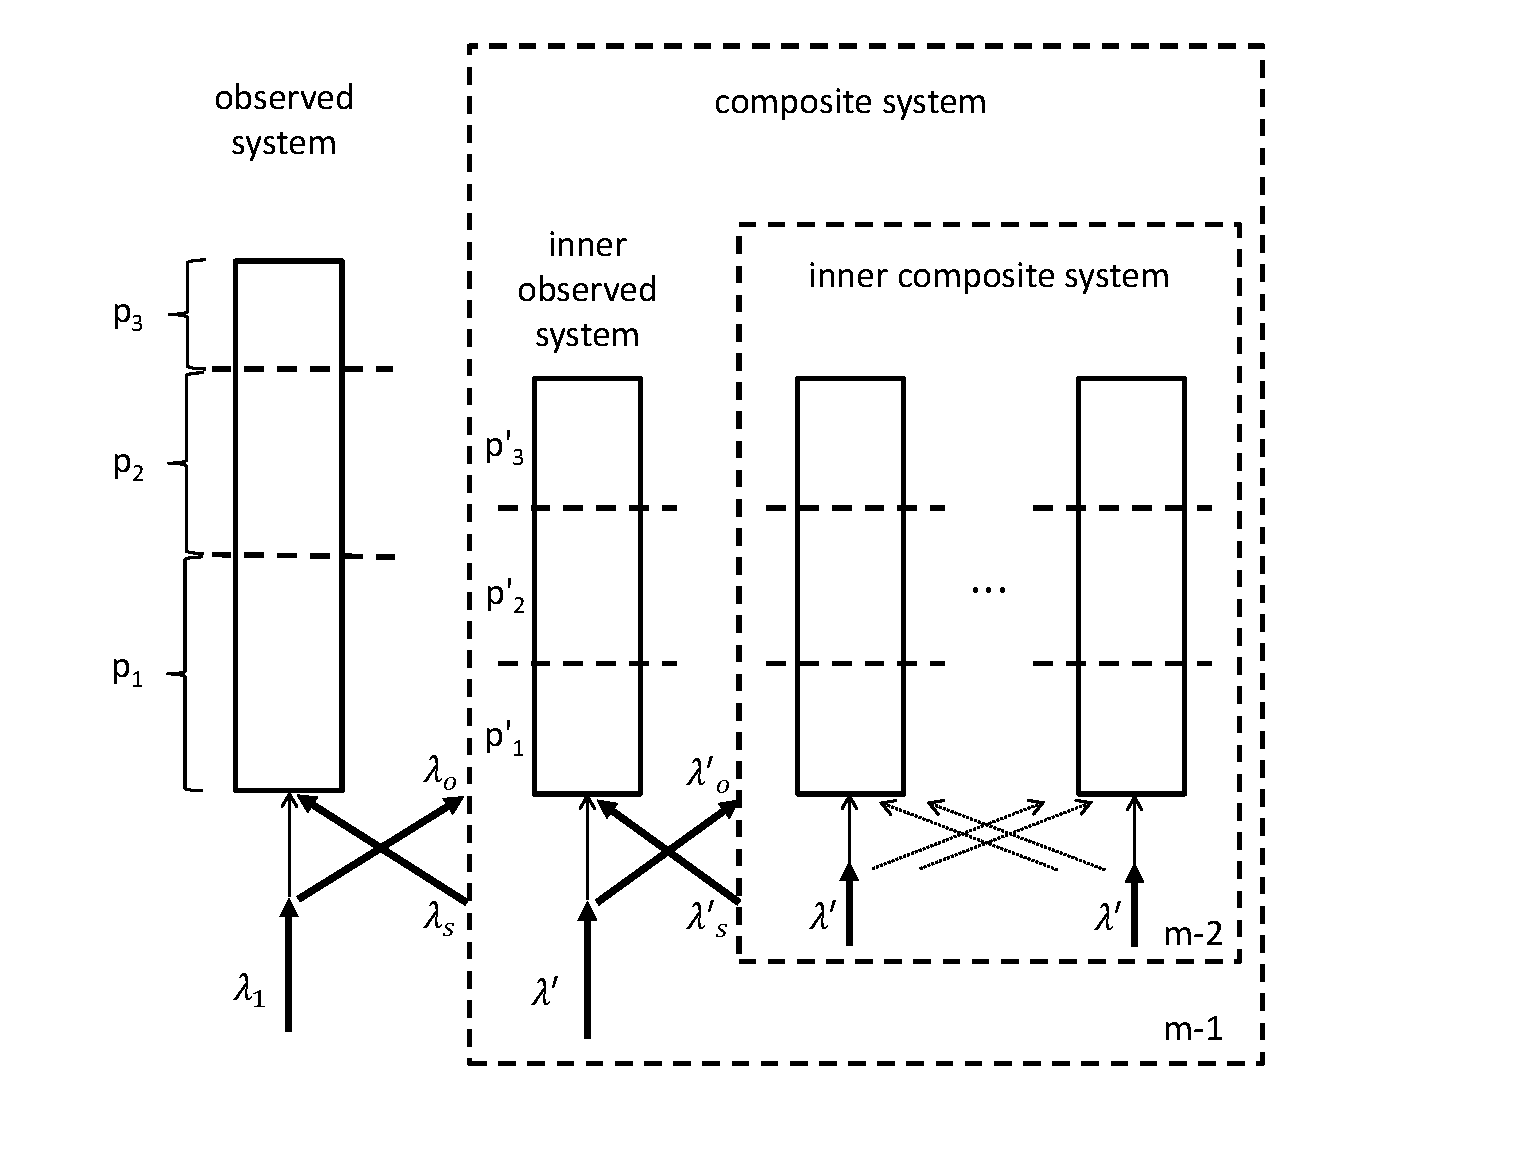
\includegraphics[width=.66\textwidth]{aggregation/performance_model/figures/composite_inner}
 	\caption{Fixed point approach for system with imbalanced load.}
 	\label{fig:composite_inner}
\end{figure}

%\begin{align}
%p_1 &= \sum x(i), & 0 \leq i < \lfloor\alpha_1\cdot n_1\rfloor \\
%p_2 &= \sum x(i), &\lfloor\alpha_1\cdot n_1\rfloor\leq i < \lfloor\beta_1\cdot n_1\rfloor \\
%p_3 &= \sum x(i), &\lfloor\beta_1\cdot n\rfloor \leq i \leq n_1
%\end{align}
%
%\begin{align}
%p'_1 &= \sum x'(i), & 0 \leq i < \lfloor\alpha'\cdot n'\rfloor \\
%p'_2 &= \sum x'(i), &\lfloor\alpha'\cdot n'\rfloor\leq i < \lfloor\beta'\cdot n'\rfloor \\
%p'_3 &= \sum x'(i), &\lfloor\beta'\cdot n\rfloor \leq i \leq n'
%\end{align}

%\small
\begin{equation}
\begin{split}
&\lambda'_{s} =\\
 &p_1\sum_{j=0}^{m-2}\sum_{k=0}^{m-2-j} \binom{m-2}{j}\binom{m-2-j}{k}p'^j_3 p'^k_1 p'^{m-2-j-k}_2\frac{j\lambda'}{k+2}+ \\
&p_2\sum_{j=0}^{m-2}\sum_{k=0}^{m-2-j} \binom{m-2}{j}\binom{m-2-j}{k}p'^j_3 p'^k_1 p'^{m-2-j-k}_2\frac{j\lambda'}{k+1} +\\
&p_3\sum_{j=0}^{m-2}\sum_{k=0}^{m-2-j} \binom{m-2}{j}\binom{m-2-j}{k}p'^j_3 p'^k_1 p'^{m-2-j-k}_2\frac{j\lambda'+\lambda_1}{k+1} \\
\end{split}
\label{eq:supportinner}
\end{equation}
%\normalsize

\begin{equation}
\lambda'_{o} = (1-(1-p_1)(1-p'_1)^{m-2})\lambda'
\label{eq:offlaodinner}
\end{equation}

In Equation~\ref{eq:supportinner}, the support rate $\lambda'_s$ is computed for the case that the inner observed system can support. The summations consider the cases that $j$ links want to offload and $k$ links can support in the inner composite system. With probability $p_1$, the outer observed system is also in support macro state, thus, in total $k+2$ systems can support (including the $k$ systems from the inner composite system and both the inner and outer observed systems) and share the offloaded traffic $j\lambda'$. With probability $p_2$, the outer observed system is in normal macro state and will not interact. However, it is in offloading macro state with probability $p_3$, which means that the offloaded traffic is increased to $j\lambda'+\lambda_1$ and shared by $k+1$ links. In contrast, the inner observed system can offload if the outer observed system is in support macro state, or at least one of the $m-2$ links of the inner composite model can help, which is reflected by Equation~\ref{eq:offlaodinner}.

%\begin{equation}
%x(i)=
%\begin{cases}
%\frac{x(i-1)(\lambda_1+\lambda_{1_s})}{i\cdot\mu}, &0\leq i < \lfloor\alpha\cdot n\rfloor \\
%\frac{x(i-1)\lambda}{i\cdot\mu}, &\lfloor\alpha\cdot n\rfloor\leq i < \lfloor\beta\cdot n\rfloor \\
%\frac{x(i-1)(\lambda_1-\lambda_{1_o})}{i\cdot\mu}, &\lfloor\beta \leq i \leq n\rfloor \\
%\end{cases} \\
%\end{equation}
%\begin{equation}
%\sum_{i=0}^n x(i) = 1
%\end{equation}
%
%
%
%\begin{equation}
%x'(i)=
%\begin{cases}
%\frac{x'(i-1)(\lambda'+\lambda'_s)}{i\cdot\mu}, &0\leq i < \lfloor\alpha'\cdot n'\rfloor \\
%\frac{x'(i-1)\lambda'}{i\cdot\mu}, &\lfloor\alpha'\cdot n'\rfloor\leq i < \lfloor\beta'\cdot n'\rfloor \\
%\frac{x'(i-1)(\lambda'-\lambda'_o)}{i\cdot\mu}, &\lfloor\beta'\cdot n'\rfloor \leq i \leq n' \\
%\end{cases} \\
%\end{equation}
%\begin{equation}
%\sum_{i=0}^{n'} x'(i) = 1
%\end{equation}

Solving this system by a joint fixed point iteration for the outer and the inner system, i.e., iterating and normalizing in turns over both systems according to Equation~\ref{eq:iteration}, will give the state probabilities $x(i)$ and $x'(i)$.%\footnote{Note that also a joint iteration yielded the same results in this case.}.

For the evaluation of this system, we will focus on the results for the outer observed link, i.e., the link that is not equal to the other $m-1$ links. For this link we will investigate the blocking probability $p_{b_1} = x(n)\cdot (1-p'_1)^{m-1}$, the received bandwidth $E[X_{A_1}] = \frac{\lambda_1}{\mu}\cdot (1-p_{b_1})$, and the bandwidth gain $\omega_1=\frac{E[X_{A_1}]-E_0[X_1]}{E_0[X_1]}$.
